\chapter{analysis}

\section{Star Tree}
	
	To do : Material on star tree, star tree analysis gives you 1 cert savings.

	\begin{figure}[H]\label{star-aggregation-tree}
  	\centering
  		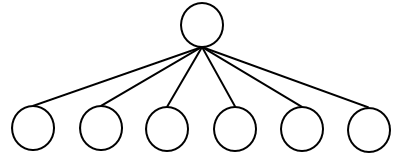
\includegraphics[scale=0.4]{images/star-tree.png}\\
  		\caption{Star aggregation tree}
  \end{figure}

\newpage

\section{Maximum savings}
	Analysis is true for any n bit forest size.	Give names to the following tolopogies.  
	\textbf{Maximum savings}, with n(=4) bit forest, fanout(=2), savings of n(=4) certificates:

	\begin{figure}[hp]
		\centering
		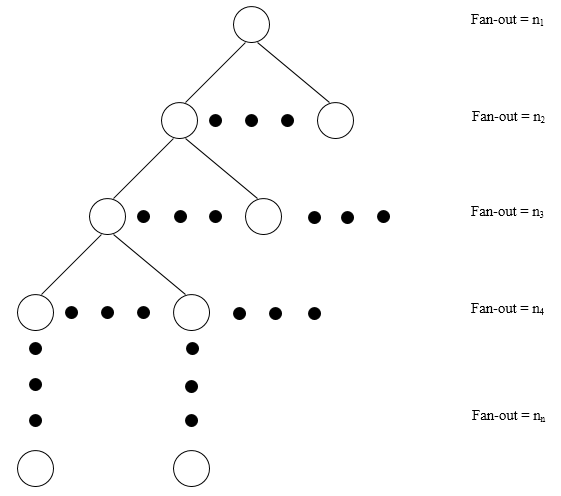
\includegraphics[scale=0.5]{images/symmetric-tree.png}\\
		\caption{Symmetric Tree}
	\end{figure}

	\begin{multicols}{2}

		\begin{tabular}{ l | l l c r }
		  1 & 1 & 1 & 1 & 0 \\
		  \hline
		  0 & 1 & 1 & 1 & 1 \\
		  0 & 1 & 1 & 1 & 1 \\
		  0 & 0 & 0 & 0 & 1 \\
		  \hline	
		  A & C & C & C & C\\
		\end{tabular}
	\columnbreak{|}
		\begin{tabular}{ l | l l c r }
		  1 & 1 & 1 & 1 & 0 \\
		  \hline
		  0 & 1 & 1 & 1 & 1 \\
		  0 & 1 & 1 & 1 & 1 \\
		  0 & 0 & 0 & 0 & 1 \\
		  \hline	
		  A & A & A & A & A\\
		\end{tabular}
	\end{multicols}

	\textbf{No savings}, with n(=4) bit forest with alternate bit positions, fanout(=2, 3, 5) :

	\begin{multicols}{3}

		\begin{tabular}{ l |l l c r }
		  
		  1 & 0 & 1 & 0 & 0 \\
		  \hline
		  0 & 1 & 0 & 1 & 0 \\
		  0 & 1 & 0 & 1 & 0 \\
		  0 & 0 & 0 & 0 & 1 \\
		  \hline	
		  A & 0 & A & 0 & A \\
		
		\end{tabular}
		\columnbreak{|}
		\begin{tabular}{ l |l l c r }
		  
		  1 & 0 & 1 & 0 & 0 \\
		  \hline
		  0 & 1 & 0 & 1 & 0 \\
		  0 & 1 & 0 & 1 & 0 \\
		  0 & 1 & 0 & 1 & 0 \\
		  0 & 0 & 0 & 0 & 1 \\
		  \hline	
		  A & C & A & C & A \\
		
		\end{tabular}
		\columnbreak{|}
		\begin{tabular}{ l l |l l c r }
		  
		  0 & 1 & 0 & 0 & 0 & 0 \\
		  0 & 1 & 0 & 1 & 0 & 0 \\
		  1 & 1 & 1 & 1 & 0 & 0 \\
		  \hline
		  0 & 0 & 1 & 0 & 1 & 0 \\
		  0 & 0 & 1 & 0 & 1 & 0 \\
		  0 & 0 & 1 & 0 & 1 & 0 \\
		  0 & 0 & 1 & 0 & 1 & 0 \\
		  0 & 0 & 1 & 0 & 1 & 0 \\
		  0 & 0 & 0 & 0 & 0 & 1 \\
		  \hline	
		  A & A & 0 & 0 & C & A \\
		
		\end{tabular}

	\end{multicols}

	\newpage

	 \textbf{Savings of n - 1 certificates}, with n(=4) bit forest, fanout(=3) :

	\begin{multicols}{2}

		\begin{tabular}{ l l |l l c r }
		  0 & 1 & 1 & 1 & 1 & 0 \\
		  1 & 1 & 1 & 1 & 1 & 0 \\
		  \hline
		  0 & 0 & 1 & 1 & 1 & 1 \\
		  0 & 0 & 1 & 1 & 1 & 1 \\
		  0 & 0 & 1 & 1 & 1 & 1 \\
		  0 & 0 & 0 & 0 & 0 & 1 \\
		  \hline	
		  A & 0 & C & C & C & 0 \\
		\end{tabular}
	\columnbreak{|}
		\begin{tabular}{ l l | l l c r }
		  0 & 1 & 1 & 1 & 1 & 0 \\
		  1 & 1 & 1 & 1 & 1 & 0 \\
		  \hline
		  0 & 0 & 1 & 1 & 1 & 1 \\
		  0 & 0 & 1 & 1 & 1 & 1 \\
		  0 & 0 & 1 & 1 & 1 & 1 \\
		  0 & 0 & 0 & 0 & 0 & 1 \\
		  \hline
		  A & 0 & A & A & A & 0\\

		\end{tabular}

	\end{multicols}

	\textbf{Savings of n - 1 certificates}, with n(=4) bit forest, fanout(=4) :

	\begin{multicols}{2}

		\begin{tabular}{ l l |l l c r }
		  
		  0 & 1 & 1 & 1 & 0 & 0 \\
		  0 & 1 & 1 & 1 & 1 & 0 \\
		  1 & 1 & 1 & 1 & 1 & 0 \\
		  \hline
		  0 & 0 & 1 & 1 & 1 & 1 \\
		  0 & 0 & 1 & 1 & 1 & 1 \\
		  0 & 0 & 1 & 1 & 1 & 1 \\
		  0 & 0 & 1 & 1 & 1 & 1 \\
		  0 & 0 & 0 & 0 & 0 & 1 \\
		  \hline	
		  A & A & C & C & 0 & C \\
		
		\end{tabular}
	\columnbreak{|}
		\begin{tabular}{ l l | l l c r }
		  0 & 1 & 1 & 1 & 0 & 0 \\
		  0 & 1 & 1 & 1 & 1 & 0 \\
		  1 & 1 & 1 & 1 & 1 & 0 \\
		  \hline
		  0 & 0 & 1 & 1 & 1 & 1 \\
		  0 & 0 & 1 & 1 & 1 & 1 \\
		  0 & 0 & 1 & 1 & 1 & 1 \\
		  0 & 0 & 1 & 1 & 1 & 1 \\
		  0 & 0 & 0 & 0 & 0 & 1 \\
		  \hline
		  A & A & A & A & 0 & A\\

		\end{tabular}

	\end{multicols}

\newpage

\section{Pseudo Palm Tree}
	\begin{figure}[hp]
		\centering
		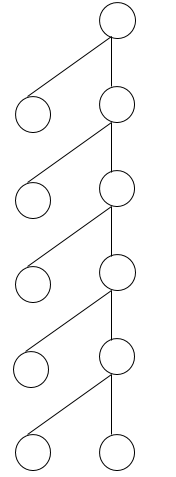
\includegraphics[scale = 0.5]{images/pseudo-palm-tree}
		\caption{Pseudo palm tree}
	\end{figure}
	
	Properties: \\
		Every aggregator has odd number of messages to aggregate, including itself.\\
		At every level you can save one certificate, if an aggregator excludes itself in the aggregation.\\
		General form of aggregation looks like the following:
	\begin{multicols}{2}
		\begin{tabular}{ l | l l l l }
			0 & 0 & 0 & 1 & 0 \\
			\hline
			0 & 0 & 0 & 0 & 1 \\
			0 & 0 & 0 & 0 & 1 \\
			X & X & X & X & 1 \\
			\hline
			X & X & X & X & C \\
		\end{tabular}
		\columnbreak{|}
		\begin{tabular}{ l | l l l l }
			0 & 0 & 0 & 1 & 0 \\
			\hline
			0 & 0 & 0 & 0 & 1 \\
			0 & 0 & 0 & 0 & 1 \\
			X & X & X & X & 1 \\
			\hline
			X & X & X & X & A \\
		\end{tabular}
	\end{multicols}

	\begin{multicols}{4}
		\begin{tabular}{ l | l }
			1 & 0 \\
			\hline
			0 & 1 \\
			0 & 1 \\
			0 & 1 \\
			\hline
			A & C \\
		\end{tabular}
		\columnbreak{|}
		\begin{tabular}{ l | l l }
			1 & 1 & 0 \\
			\hline
			0 & 0 & 1 \\
			0 & 0 & 1 \\
			0 & 1 & 1 \\
			\hline
			A & 0 & C \\
		\end{tabular}
		\columnbreak{|}
		\begin{tabular}{ l l l }
			0 & 1 & 0 \\
			\hline
			0 & 0 & 1 \\
			0 & 0 & 1 \\
			1 & 0 & 1 \\
			\hline
			C & A & C \\
		\end{tabular}
		\columnbreak{|}
		\begin{tabular}{ l | l l l }
			1 & 1 & 1 & 0 \\
			\hline
			0 & 0 & 0 & 1 \\
			0 & 0 & 0 & 1 \\
			0 & 1 & 1 & 1 \\
			\hline
			A & 0 & 0 & C \\
		\end{tabular}
	\end{multicols}

	\begin{multicols}{4}
		\begin{tabular}{ l | l }
			1 & 0 \\
			\hline
			0 & 1 \\
			0 & 1 \\
			0 & 1 \\
			\hline
			A & A \\
		\end{tabular}
		\columnbreak{|}
		\begin{tabular}{ l | l l }
			1 & 1 & 0 \\
			\hline
			0 & 0 & 1 \\
			0 & 0 & 1 \\
			0 & 1 & 1 \\
			\hline
			A & 0 & A \\
		\end{tabular}
		\columnbreak{|}
		\begin{tabular}{ l l l }
			0 & 1 & 0 \\
			\hline
			0 & 0 & 1 \\
			0 & 0 & 1 \\
			1 & 0 & 1 \\
			\hline
			C & A & A \\
		\end{tabular}
		\columnbreak{|}
		\begin{tabular}{ l | l l l }
			1 & 1 & 1 & 0 \\
			\hline
			0 & 0 & 0 & 1 \\
			0 & 0 & 0 & 1 \\
			0 & 1 & 1 & 1 \\
			\hline
			A & 0 & 0 & A \\
		\end{tabular}
	\end{multicols}

Meeting:

	Find cases where you can say it will be always A's.
	Analyze palm tree / pseudo palm tree 